\documentclass{article}

% Packages
\usepackage{amsmath} % For math equations
\usepackage{amssymb} % For math symbols
\usepackage{geometry} % For page layout
\usepackage{fancyhdr} % For headers and footers
\usepackage{lipsum} % For dummy text (remove this line)
\usepackage{float}
\usepackage{listings}
\usepackage{xcolor}
\usepackage{graphicx}
\usepackage{array} % 导入 array 宏包
\usepackage{verbatim} % 导入 verbatim 宏包
\usepackage{calc}
\usepackage{slashbox}
\usepackage{pict2e}
\usepackage[utf8]{inputenc}
\usepackage{circuitikz}

% Set the page margins
\geometry{margin=1in}
% Set the top margins
\addtolength{\topmargin}{-.5in}
\title{Digital System Assignment 3}
\author{He Tianyang}
\date{\today}



\begin{document}
\maketitle

\section{Problem 1}
Utilize an 8-bit Mux CT74LS151 for the implementation of a 4-bit even-odd checker. The input consists of a 4-bit binary number, producing an output of 1 if the count of 1s in the input is even, and 0 if it is odd. Refer to the truth table provided below. Additionally, furnish the circuit diagram along with comprehensive design steps.
\\
\textbf{Solves:}

First, we need to design the truth table of the 4-bit even-odd checker. The truth table is shown below.

\begin{table}[H]
    \centering
    \begin{tabular}{|c|c|}
        \hline
        Input & Output \\
        \hline
        0000  & 1      \\
        0001  & 0      \\
        0010  & 0      \\
        0011  & 1      \\
        0100  & 0      \\
        0101  & 1      \\
        0110  & 1      \\
        0111  & 0      \\
        1000  & 0      \\
        1001  & 1      \\
        1010  & 1      \\
        1011  & 0      \\
        1100  & 1      \\
        1101  & 0      \\
        1110  & 0      \\
        1111  & 1      \\
        \hline
    \end{tabular}
\end{table}

Based on the truth table, we can draw the Karnaugh map of the 4-bit even-odd checker using dimension reduction method. The K-map is shown below.

\begin{table}[H]
    \centering
    \begin{tabular}{|c|c|c|}
        \hline
        \backslashbox{AB}{C} & 0              & 1              \\\hline
        00                   & $\overline{D}$ & $D$            \\\hline
        01                   & $D$            & $\overline{D}$ \\\hline
        11                   & $\overline{D}$ & $D$            \\\hline
        10                   & $D$            & $\overline{D}$ \\\hline
    \end{tabular}
\end{table}

Therefore, the circuit diagram of the 4-bit even-odd checker is shown in Figure \ref{fig:4-bit-even-odd-checker}.

\begin{figure}[H]
    \centering
    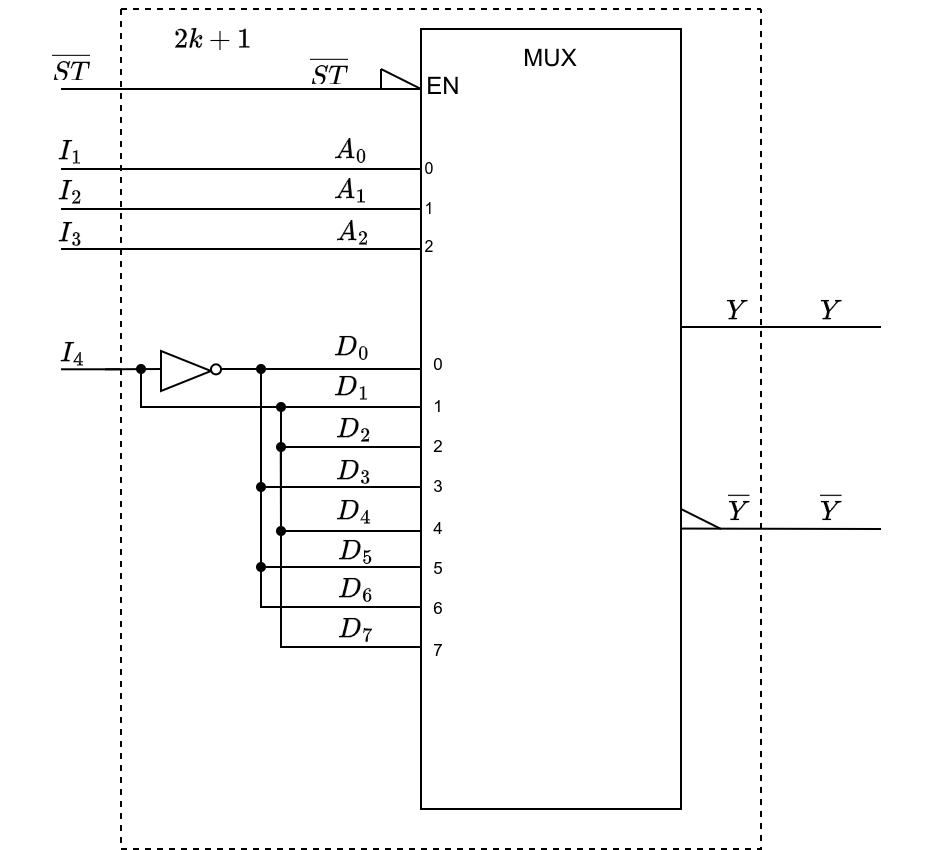
\includegraphics[width=0.7\textwidth]{./image/mux_2k+1.png}
    \caption{Circuit diagram of the 4-bit even-odd checker.}
    \label{fig:4-bit-even-odd-checker}
\end{figure}

\end{document}